%% ACLing 2026 submission (anonymous review version).
%% Built on the official ACLing 2026 / Procedia Computer Science LaTeX template
%% (elsarticle.cls + ecrc.sty, unmodified). Compile with pdfLaTeX.
\documentclass[3p,times,procedia]{elsarticle}
\flushbottom

\usepackage{ecrc}
\usepackage[bookmarks=false]{hyperref}
    \hypersetup{colorlinks,
      linkcolor=blue,
      citecolor=blue,
      urlcolor=blue}

\volume{00}
\firstpage{1}
\journalname{Procedia Computer Science}
\runauth{Anonymous}
\jid{procs}

\usepackage{amssymb}
\usepackage{amsmath}
\usepackage[T1]{fontenc}
\usepackage[safe]{tipa}

%% ---- Sinhala examples ---------------------------------------------------
%% Sinhala text is set as small vector PDFs (one per word) so that the paper
%% compiles with pdfLaTeX. Each glyph is followed by its IPA in brackets.
\makeatletter
\newcommand{\sinhalaglyph}[1]{%
  \raisebox{-0.25\height}{%
    \includegraphics[height=1.2\dimexpr\f@size pt\relax]{sinhala/#1}}}
\makeatother
\newcommand{\siex}[2]{\sinhalaglyph{#1}\,[\textipa{#2}]}
\newcommand{\sikohomada}{\siex{si-kohomada}{k6h6m2D2}}
\newcommand{\sitha}{\siex{si-tha}{T2}}
\newcommand{\siwa}{\siex{si-wa}{v2}}
\newcommand{\sika}{\siex{si-ka}{k2}}
\newcommand{\sikaa}{\siex{si-kaa}{ka:}}
\newcommand{\sikhal}{\siex{si-khal}{k}}

\newcommand{\rom}[1]{\textit{#1}}
\newcommand{\anonrepo}{\url{https://anonymous.4open.science/r/sinhala-script-robustness-llm}}


\begin{document}
\begin{frontmatter}

\dochead{8th International Conference on AI in Computational Linguistics}

\title{Does Script Choice Matter for Sinhala? A Tokenizer-Independent Re-evaluation and a Paired Downstream Study of Open Language Models}

\author[a]{Anonymous Author(s)}
\address[a]{Affiliation withheld for double-blind review}

\begin{abstract}
Formal Sinhala is written in its own script, but much informal writing online is in Romanized Sinhala, which uses Latin letters. A recent benchmark used perplexity to report that open language models are about 312 times worse on Romanized Sinhala than on the Sinhala script. Perplexity is an average over tokens, and tokenizers split the same Sinhala sentence into very different numbers of tokens. We re-score 31 open models (0.35B to 14.7B parameters) on the same 500 parallel sentences and reproduce the published perplexities of the 24 shared models to a median of 0.05\%. We then count bits per word, because the word is the only text unit with the same count in both scripts. In this unit almost all of the 312-fold ratio comes from the change in token count, and the median model assigns only 6\% more bits to the Romanized version of a sentence. We also test eleven instruction-tuned models on SinhalaMMLU and SOLD in both scripts. Romanization lowers the scores of the stronger models, shrinks the spread between models on SinhalaMMLU from 22.4 to 6.7 points, and removes about half of the offensive-language detection signal, even though the Romanized input is shorter in tokens for every model.
\end{abstract}

\begin{keyword}
Sinhala; Romanized text; tokenization; perplexity; bits per byte; low-resource evaluation; language models
\end{keyword}
\end{frontmatter}

%% =========================================================================
\section{Introduction}
\label{sec:intro}

Sinhala is an Indo-Aryan language spoken by more than 17 million people, almost all of them in Sri Lanka \cite{desilva-survey,sold}. Formal writing uses the Sinhala script, but chat and social media posts are often in Romanized Sinhala, informally called Singlish in Sri Lanka, which has no standard spelling. For example, \sikohomada{} (``how are you'') can be typed as \rom{kohomada}, \rom{kohomd} or \rom{kohomade}. Almost all Sinhala benchmarks are in the Sinhala script \cite{sinhalammlu,sold}, so a model can score well on them without being tested on the form of the language that many users type.

Rajapakse and Weerasinghe \cite{rajapakse} were the first to measure this gap. They scored 24 open models with perplexity on 500 parallel sentences. They reported that the median model has a 312 times higher perplexity on Romanized text than on the Sinhala script, and that model size is not related to how well a model handles either script. Perplexity is the exponential of the average loss per token. Across the models we study, a Sinhala-script word takes 4.3 to 14.2 tokens, while its Romanized form takes about two. A perplexity ratio between the scripts therefore mixes the probability a model gives to the text with the number of tokens the text was cut into. Rajapakse and Weerasinghe also noted that perplexity does not show whether a model can still do useful work, and called for downstream tests. This paper takes up both points. We re-score the same sentences with metrics that divide by a property of the text, split the reported ratio exactly into a token-count part and a content part, and test eleven instruction-tuned models on 9{,}379 downstream items in both scripts. We release our Sinhala-to-Latin transliterator with all code and model outputs.

%% =========================================================================
\section{Related Work}
\label{sec:related}

Sinhala is a low-resource language \cite{ranathunga-desilva}. Its recent evaluation sets, such as SinhalaMMLU \cite{sinhalammlu} and the Sinhala Offensive Language Dataset (SOLD) \cite{sold}, use only the Sinhala script. Work on Romanized Sinhala has mostly trained task models for it \cite{emoscan,chamikara}, and Sinhala transliteration tools mostly convert Latin into Sinhala script \cite{demel,swabhasha}. The Swa-bhasha Resource Hub \cite{swabhasha} collects human-written Romanized Sinhala, with an average of 15.7 accepted spellings per word.

For other South Asian languages, Romanized text has been studied mainly as a data and language identification problem \cite{dakshina}. RomanSetu \cite{romansetu} shows that romanization can help a model trained for it, while we study models without such training. Khullar et al. \cite{scriptgap} found that model triage of real Hindi and Telugu health messages was worse on Romanized ones, the closest result to ours.

Bits per byte is used to compare models whose tokenizers cut text differently \cite{pile,paloma}. Tokenizers are known to treat languages unequally \cite{petrov,ahia,velayuthan}. Sinhala-specific vocabularies, such as those of HelaBERT \cite{helabert} and SinLlama \cite{sinllama}, reduce this problem for the Sinhala script.

%% =========================================================================
\section{Experimental Setup}
\label{sec:setup}

The design follows one rule. Between the two test conditions, only the script changes. Every comparison is made within one model and over the same content.

\subsection{Data and romanization}
\label{sec:translit}

For the intrinsic measurements we use the 500 parallel sentence pairs released by Rajapakse and Weerasinghe \cite{rajapakse}. Native speakers typed the Romanized side, so these measurements do not depend on our transliterator.

For the downstream tests we use every item of two tasks, with no sampling. SinhalaMMLU \cite{sinhalammlu} is a multiple-choice benchmark in the style of MMLU \cite{mmlu}, with 6{,}879 items over six subject domains and three difficulty levels. Of these, 2{,}145 items have five options and the rest have four, so random guessing scores 23.4\%. We obtained the full set from its authors, since the public release has 1{,}851 items. SOLD \cite{sold} is a binary offensive language detection task. Its 2{,}500-item test split has 40.6\% offensive posts, so always predicting ``not offensive'' gives 59.4\% accuracy. This gives 9{,}379 items and 18{,}758 prompts per model.

No human-written Romanized version of these tasks exists, so we wrote a rule-based Sinhala-to-Latin transliterator. Sinhala is an abugida. A consonant letter carries a default vowel, so \sika{} is \rom{ka}. A vowel sign changes the vowel, as in \sikaa{} \rom{kaa}, and another sign removes it, as in \sikhal{} \rom{k}. The transliterator reads these units and writes them the way people commonly type, for example \sitha{} as \rom{th} and \siwa{} as \rom{w}. We compared four methods, namely ours, Aksharamukha \cite{aksharamukha}, uroman \cite{uroman}, and the web romanizer released with the Sinhala part of Global PIQA \cite{desilva-piqa}. The references were three human-written sets from the Swa-bhasha Resource Hub \cite{swabhasha}, with 4{,}397 social media sentences, 450{,}587 lexicon words and 300{,}000 machine-augmented sentences. Against the closest accepted spelling, our character error rates are 0.182, 0.121 and 0.112 on the three sets. The next best method, Aksharamukha, scores 0.191, 0.148 and 0.139, and a paired Wilcoxon test separates ours from each other method at $p < 0.001$ on the two large sets. Most remaining errors come from writing long vowels as double letters (\rom{ee}, \rom{aa}), which all four methods do more often than people. Once doubled vowels are merged, 88.6\% of our word tokens on the parallel corpus use a spelling that some person gave for that word in the Swa-bhasha lexicon. For the native speakers' text it gives 84.2\%.

\subsection{Models, prompts and statistics}
\label{sec:screen}

The intrinsic evaluation covers 31 decoder-only models from 0.35B to 14.7B parameters, from the Llama \cite{llama3}, Qwen \cite{qwen2,qwen3}, Gemma \cite{gemma2}, Mistral, BLOOM \cite{bloom}, OPT, Pythia \cite{pythia}, Phi \cite{phi4} and other families. Twenty-four are exactly the models of Rajapakse and Weerasinghe \cite{rajapakse}. We added three newer base models and four instruction-tuned models. The downstream tests use the eleven instruction-tuned models in Table~\ref{tab:main}, because they need a model that follows an answer format. The repository lists their Hugging Face identifiers.

Downstream prompts are zero-shot, with an English instruction and the item in Sinhala, so only the item text changes between conditions. Each prompt goes through the model's chat template, and decoding is greedy with at most 40 new tokens. We picked the template from three candidates in a small pilot (nine models, both scripts, 20 items per task). It was the only one that never gave an unreadable answer on SinhalaMMLU, and we used it for both tasks. Answers are read with a fixed pattern, and an unreadable answer counts as wrong.

All tests are paired. For accuracy we use McNemar's test with continuity correction \cite{mcnemar}, and for the Matthews correlation coefficient (MCC) on SOLD and all confidence intervals a paired bootstrap with 10{,}000 resamples. Within each task we correct $p$-values across models with Holm's method \cite{holm}. We report MCC for SOLD because its classes are unbalanced, so accuracy stays near the majority baseline even for a model that has learned little \cite{matthews}.

A model that only guesses in the Sinhala script has nothing to lose under romanization, so its gap is near zero for that reason alone. Averaging such models with the others pulls the average gap towards zero. We therefore call a model \emph{competent} on SinhalaMMLU if its Sinhala-script accuracy is above chance at $p < 0.01$ and it gives the same option for no more than 90\% of the items. Six of the eleven models pass. All eleven appear in every table.

%% =========================================================================
\section{Intrinsic Evaluation}
\label{sec:intrinsic}

\subsection{Metrics and reproduction}

For each model and script we add up the negative log-likelihood of all 500 sentences in bits, $N$. Bits per byte (BPB) divides $N$ by the number of UTF-8 bytes, bits per character (BPC) by Unicode code points, and bits per word (BPW) by whitespace-separated words. They remove the token count from the denominator, but $N$ still depends on the tokenizer.

Within one script the unit does not matter for comparing models, because all models see the same text, so BPB, BPC and BPW rank them in the same order. The unit matters only when the two scripts are compared. The Sinhala side has 43{,}152 bytes and 16{,}278 code points, while the Romanized side has 18{,}731 bytes and 18{,}679 code points, because most Sinhala code points take three bytes in UTF-8 and Latin letters take one. Only the word count, 3{,}035, is the same. We therefore use bits per word whenever we compare the two scripts.

Our perplexities reproduce the published values for all 24 shared models, with a median absolute difference of 0.05\% on the Sinhala script and 0.004\% on Romanized text, and our median ratio is also 312.3. Any change in the conclusions below therefore comes from the metric, not from a different run.

\subsection{Perplexity mostly measures the tokenizer}

Across the 31 models, Sinhala-script perplexity and Sinhala-script BPB are not related (Spearman $\rho = 0.08$, $p = 0.68$). Gemma-2-9B ranks 26th by perplexity and 2nd by BPB. Figure~\ref{fig:intrinsic}a shows why. Perplexity closely follows the number of tokens that the tokenizer uses per Sinhala word ($\rho = -0.87$, $p < 10^{-9}$). Cutting the same sentence into more tokens lowers the loss per token even if the sentence gets the same probability.

This changes the finding about model size. Parameter count is not related to Sinhala-script perplexity ($\rho = 0.15$, $p = 0.42$), in line with Rajapakse and Weerasinghe. It is related to Sinhala-script BPB ($\rho = -0.55$, $p = 0.001$), and this also holds on their 24 models alone ($\rho = -0.42$, $p = 0.04$). On Romanized text the relation is weaker and not significant ($\rho = -0.28$, $p = 0.13$). The models differ in family, tokenizer and training data at once, so this is an association across models and not a scaling law.

\begin{figure}[t]
\centering
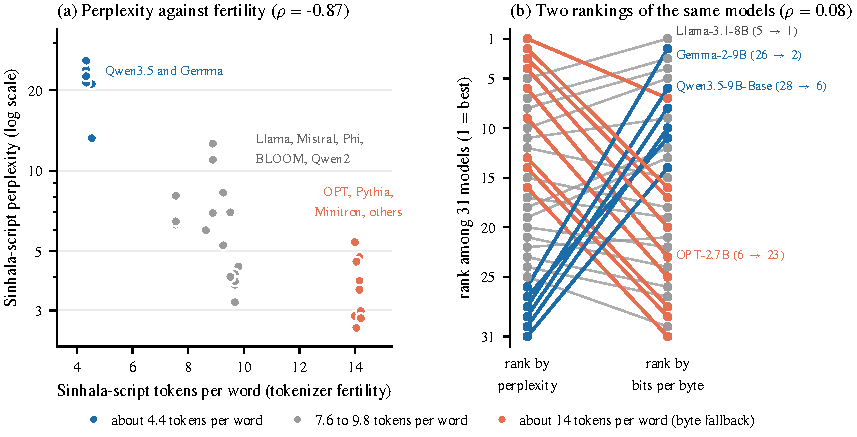
\includegraphics[width=\textwidth]{figures/fig1_intrinsic.pdf}
\caption{Intrinsic results for the 31 models on the 500 parallel sentences. (a) Sinhala-script perplexity against the tokens each tokenizer uses per Sinhala word. (b) Bits per word for the same sentences in each script. Points below the dashed line assign fewer bits to the Romanized version. The arrow goes from Llama-3-8B to SinLlama, which is the same model with Sinhala tokens added and further training on Sinhala.}
\label{fig:intrinsic}
\end{figure}

\subsection{Where the 312-fold ratio comes from}
\label{sec:decomp}

Let $T$ be the number of tokens and $U$ the number of text units. For one model and one script, $\log_2 \mathrm{PPL} = N/T = (N/U)(U/T) = b\,x$, where $b$ is bits per unit and $x$ is units per token. The change from the Sinhala script ($s$) to Romanized text ($r$) then splits exactly into two terms,
\begin{equation}
\log_2 \frac{\mathrm{PPL}_r}{\mathrm{PPL}_s} \;=\; \underbrace{\bar{b}\,(x_r - x_s)}_{\text{token count}} \;+\; \underbrace{\bar{x}\,(b_r - b_s)}_{\text{content}},
\label{eq:decomp}
\end{equation}
where $\bar{b}$ and $\bar{x}$ are the averages of the two scripts. The first term is the change caused only by cutting the text into a different number of tokens. The second is the change in bits per unit of text.

This identity holds for any unit, but the split depends on which unit is used. With bytes, the change in byte count between the scripts is partly counted as a change in content. Table~\ref{tab:decomp} gives the split for three units. Medians of the two terms do not add up to the median of the total, so the table reports means of $\log_2$ ratios, which do add up. On the 24 models of Rajapakse and Weerasinghe, the token-count term explains 46\% of the mean ratio when the unit is bytes and 114\% when it is code points. With words, the only unit with the same count in both scripts, it explains 102\%, and the content term is close to zero.

\begin{table}[t]
\caption{Exact split of the mean $\log_2$ perplexity ratio (Romanized over Sinhala script) by Equation~\ref{eq:decomp}, for three text units. Values are means over models, in bits. The mean $\log_2$ ratio is 8.39 bits on the 24 models of \cite{rajapakse} and 8.06 on all 31. ``Share'' is the token-count term as a percentage of it.}
\label{tab:decomp}
\begin{tabular*}{\hsize}{@{\extracolsep{\fill}}lrrrrrrrr@{}}
\toprule
& \multicolumn{2}{c}{Units in corpus} & \multicolumn{3}{c}{24 models of \cite{rajapakse}} & \multicolumn{3}{c}{All 31 models} \\
\cline{2-3}\cline{4-6}\cline{7-9}
Unit & Sinhala & Romanized & Token count & Content & Share & Token count & Content & Share \\
\colrule
Byte & 43{,}152 & 18{,}731 & 3.88 & 4.51 & 46\% & 3.15 & 4.91 & 39\% \\
Code point & 16{,}278 & 18{,}679 & 9.53 & $-1.14$ & 114\% & 8.97 & $-0.91$ & 111\% \\
Word & 3{,}035 & 3{,}035 & 8.56 & $-0.17$ & 102\% & 8.00 & 0.06 & 99\% \\
\botrule
\end{tabular*}
\end{table}

Figure~\ref{fig:intrinsic}b compares bits per word directly. The median model assigns 1.1 more bits per word (6\% more in total) to the Romanized version of a sentence, and 12 of the 31 models assign fewer. On this corpus, then, the 312-fold ratio comes almost entirely from the token count and does not show that the models give much less probability to Romanized Sinhala. The content term still depends on each model's tokenizer, so Equation~\ref{eq:decomp} removes the effect of the token count, not every effect of tokenization.

Figure~\ref{fig:intrinsic}b also shows a pattern that returns downstream. Sinhala-script cost ranges from 16.3 to 34.1 bits per word across models, but Romanized cost only from 20.3 to 25.7. In a linear fit, one bit per word of improvement on the Sinhala script goes with only 0.14 bits on Romanized text ($R^2 = 0.19$). So the models best on the Sinhala script have the largest per-word gap ($\rho = -0.88$, $p < 10^{-9}$).

\subsection{A model adapted to Sinhala}
\label{sec:sinllama}

SinLlama \cite{sinllama} adds 11{,}080 Sinhala tokens to Llama-3-8B and continues its training on Sinhala text. We scored it and its exact base model. On the Sinhala script the adaptation works, and the cost falls from 16.4 to 8.9 bits per word, the lowest of the 32 models we scored. Perplexity rises from 3.25 to 74.56 because a Sinhala word now takes 1.44 tokens instead of 9.68. The perplexity ratio between the scripts falls from 311 to 8.7, the smallest we measured, so by perplexity SinLlama looks like the most balanced model. Per word the opposite is true. Its Romanized cost improves only from 22.2 to 20.8 bits per word, so the gap between the scripts grows from 5.8 to 11.9 bits per word, the largest of all 32.

%% =========================================================================
\section{Downstream Evaluation}
\label{sec:extrinsic}

The intrinsic results do not show whether a model can still answer questions or classify posts. Table~\ref{tab:main} compares each model's answers to the same items in the two scripts.

\begin{table}[t]
\caption{Downstream results, ordered by model size. ``Sinh.'' is the Sinhala-script condition and ``Rom.'' the Romanized one. For SinhalaMMLU, $\Delta$ is Sinhala-script minus Romanized accuracy in points, with its 95\% paired bootstrap interval (not corrected for multiple testing) and the Holm-corrected McNemar $p$-value. For SOLD, $p$ is for the change in MCC (paired bootstrap, Holm). Unreadable answers count as wrong, which explains the very low SOLD accuracy of the two smallest models. $^{*}$ marks models passing the competence screen.}
\label{tab:main}
{\footnotesize
\begin{tabular*}{\hsize}{@{\extracolsep{\fill}}lrrrrcrrrrrr@{}}
\toprule
& & \multicolumn{5}{c}{SinhalaMMLU (6{,}879 items)} & \multicolumn{5}{c}{SOLD (2{,}500 items)} \\
\cline{3-7}\cline{8-12}
& Size & \multicolumn{2}{c}{Accuracy (\%)} & & & & \multicolumn{2}{c}{Accuracy (\%)} & \multicolumn{2}{c}{MCC} & \\
\cline{3-4}\cline{8-9}\cline{10-11}
Model & (B) & Sinh. & Rom. & $\Delta$ & 95\% CI & $p_{\text{Holm}}$ & Sinh. & Rom. & Sinh. & Rom. & $p_{\text{Holm}}$ \\
\colrule
TinyLlama-1.1B-Chat & 1.1 & 21.7 & 21.9 & $-$0.2 & [$-$0.5, 0.1] & .8273 & 4.2 & 22.3 & $-$0.019 & $-$0.043 & 1.000 \\
LaMini-GPT-1.5B & 1.5 & 0.9 & 18.8 & $-$17.9 & [$-$18.8, $-$16.9] & $<$.0001 & 3.4 & 32.2 & 0.000 & 0.024 & 1.000 \\
StableLM-Zephyr-3B & 2.8 & 22.9 & 24.0 & $-$1.1 & [$-$2.3, 0.1] & .4275 & 59.6 & 59.0 & 0.036 & 0.001 & .9408 \\
SmolLM3-3B & 3.1 & 25.1 & 25.5 & $-$0.3 & [$-$1.0, 0.4] & .8273 & 40.9 & 40.9 & 0.025 & 0.017 & 1.000 \\
Qwen3.5-4B$^{*}$ & 4.0 & 36.7 & 26.1 & +10.6 & [9.3, 12.0] & $<$.0001 & 60.5 & 55.2 & 0.219 & 0.127 & .0018 \\
Zephyr-7B-beta & 7.2 & 24.3 & 24.9 & $-$0.6 & [$-$1.7, 0.5] & .8273 & 59.7 & 59.8 & 0.060 & 0.060 & 1.000 \\
Qwen2-7B-Instruct$^{*}$ & 7.6 & 29.0 & 27.0 & +2.0 & [0.8, 3.2] & .0055 & 61.9 & 56.8 & 0.148 & 0.042 & .0018 \\
Llama-3.1-8B-Instruct$^{*}$ & 8.0 & 32.5 & 27.1 & +5.4 & [4.1, 6.7] & $<$.0001 & 65.8 & 59.7 & 0.259 & 0.105 & $<$.0001 \\
Hormoz-8B$^{*}$ & 8.0 & 26.0 & 25.2 & +0.8 & [$-$0.5, 2.0] & .8273 & 60.7 & 59.1 & 0.108 & 0.090 & 1.000 \\
Qwen3.5-9B$^{*}$ & 9.0 & 44.1 & 28.7 & +15.5 & [14.0, 16.9] & $<$.0001 & 63.3 & 52.0 & 0.280 & 0.069 & $<$.0001 \\
Phi-4-14B$^{*}$ & 14.7 & 28.7 & 27.2 & +1.5 & [0.2, 2.8] & .1286 & 54.5 & 50.9 & 0.152 & 0.076 & .0084 \\
\botrule
\end{tabular*}}
\end{table}

\subsection{Multiple-choice knowledge (SinhalaMMLU)}

Four of the six competent models lose significantly when the questions are romanized. Qwen3.5-9B falls from 44.1\% to 28.7\%, a drop of 15.5 points. Qwen3.5-4B loses 10.6 points, Llama-3.1-8B-Instruct 5.4 and Qwen2-7B-Instruct 2.0. Hormoz-8B and Phi-4-14B are only 2.5 and 5.2 points above chance in the Sinhala script, and their smaller losses are not significant after correction. Over the six competent models the drop is 6.0 points (95\% CI 5.4 to 6.5). A logistic regression on item-level answers (model fixed effects, item-clustered errors) gives an odds ratio of 0.70 for a correct answer under romanization ($p < 0.001$). The other five models are near chance in the Sinhala script. LaMini-GPT-1.5B gives an unreadable answer to 95.9\% of the Sinhala-script items, so its apparent gain under romanization is a formatting effect.

\begin{figure}[t]
\centering
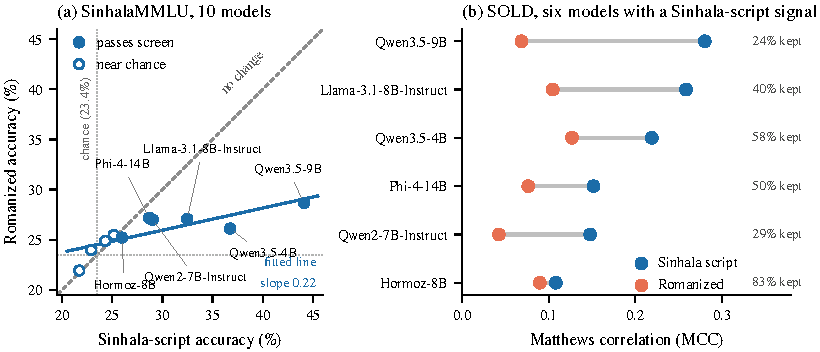
\includegraphics[width=\textwidth]{figures/fig2_downstream.pdf}
\caption{Downstream results in both scripts. (a) SinhalaMMLU accuracy for ten models. LaMini-GPT-1.5B is left out because 95.9\% of its Sinhala-script answers were unreadable. Filled points pass the competence screen. The solid line is the least-squares fit (slope 0.22). A slope of 1 would mean that the whole Sinhala-script advantage carries over to Romanized text. (b) SOLD MCC for the six models with a Sinhala-script MCC above 0.1, with the share kept after romanization.}
\label{fig:downstream}
\end{figure}

\subsection{How much of a model's advantage carries over}
\label{sec:transfer}

In the Sinhala script, the ten models with readable answers span 22.4 points on SinhalaMMLU. Under romanization they span 6.7 points, and the best model is only 5.3 points above chance (Figure~\ref{fig:downstream}a). A least-squares fit of Romanized on Sinhala-script accuracy has a slope of 0.22 (95\% CI 0.11 to 0.54, $R^2 = 0.65$). Each extra point of Sinhala-script accuracy goes with only about 0.22 points of Romanized accuracy, well below the slope of 1 for full carry-over ($p < 10^{-6}$). Refitting with one model left out at a time gives slopes between 0.17 and 0.26, so no single model drives the result. We regress Romanized accuracy on Sinhala-script accuracy rather than the drop on Sinhala-script accuracy, because the drop contains Sinhala-script accuracy and would correlate with it even with no real relation.

Since ten models is a small sample, we repeated the fit over the 16 non-empty domain and difficulty groups of SinhalaMMLU items. Pooling the six competent models within each group gives a slope of 0.45 (95\% CI 0.36 to 0.63, $R^2 = 0.75$), again well below 1. The two fits use the same outputs and are not independent, but they agree. By difficulty level the drop is 7.9 points on Easy, 6.2 on Medium and 4.3 on Hard items, where models are nearer chance.

\subsection{Offensive language detection (SOLD)}

Six models have a Sinhala-script MCC above 0.1 on SOLD. The other five have an MCC of 0.06 or lower. For the six, romanization lowers accuracy by 1.6 to 11.3 points, a moderate change next to the 59.4\% majority baseline. MCC falls much more (Figure~\ref{fig:downstream}b). Qwen3.5-9B keeps 24\% of its MCC, Qwen2-7B-Instruct 29\% and Llama-3.1-8B-Instruct 40\%, and the median model keeps 45\%. Five of the six losses are significant after correction, the exception being Hormoz-8B. Part of the loss is a shift in the predicted label. Qwen2-7B-Instruct labels 10.5\% of posts as offensive in the Sinhala script and 23.4\% after romanization. Judged by accuracy alone, it would look like a small change.

\subsection{Checks on the downstream result}
\label{sec:controls}

\textit{Input length.} Most of these tokenizers fall back to bytes for the Sinhala script, so every model receives fewer tokens in the Romanized condition on both tasks (median ratio 0.48 on SinhalaMMLU). We also split the SinhalaMMLU items into three equal groups by how much romanization shortened them. If token count drove the loss, it would change steadily across the groups, but the pooled losses are 5.1, 6.6 and 6.2 points.

\textit{Answer collapse.} A model could fall to chance by always giving the same answer. The competent models put, on average, 37.3\% of their answers on their most frequent option in the Sinhala script and 39.8\% after romanization (Wilcoxon $p = 0.31$), and at most 0.03\% of their answers are unreadable. They are simply wrong more often.

\textit{Spelling of the transliteration.} On the 500 parallel sentences, six of the smaller models assign 3.2 to 3.7 more bits per word to our transliteration than to the native speakers' typing, so our text is harder to predict. How downstream accuracy would change on human-typed items is unknown. As a partial check, we split the SOLD items into three groups by how often their Romanized words match a human spelling in the Swa-bhasha lexicon. If unusual spellings caused the loss, the least human-like group should lose most. Pooled over the five models with a significant MCC loss, it loses least, with accuracy drops of 5.0, 7.2 and 7.3 points from the least to the most human-like group. Per item, match rate and loss are unrelated ($\rho = 0.02$, $n = 2{,}447$).

\textit{Intrinsic predictors.} Over the ten models, those with lower Sinhala-script BPB lose more on SinhalaMMLU ($\rho = -0.83$, $p = 0.003$) and more MCC on SOLD ($\rho = -0.78$, $p = 0.008$). Neither the per-word gap between the scripts ($\rho = 0.45$, $p = 0.19$) nor the perplexity ratio ($\rho = -0.52$, $p = 0.13$) is related to the SinhalaMMLU loss. With ten models this is a first indication only.

%% =========================================================================
\section{Limitations}

All results are for Sinhala, zero-shot prompting with one English instruction template, greedy decoding, and open models up to 14.7B parameters. Few-shot prompting, back-transliteration or fine-tuning on Romanized text may reduce the gaps and were not tested. The downstream Romanized items are machine transliterated. Language models find them harder to predict than human typing, so the downstream gaps apply to this transliterated input. The models differ in family, tokenizer and training data at once, so the size association is not causal. Most training data are not public, so we cannot check exposure to Romanized Sinhala or test-set contamination.

%% =========================================================================
\section{Conclusion}

Perplexity ratios between the Sinhala script and Romanized Sinhala mostly reflect how differently tokenizers cut the two scripts. Counted per word, almost all of the reported 312-fold ratio comes from the token count. With this measurement, larger models do better on the Sinhala script, while their Romanized cost changes little. Downstream, on our transliterated items, the stronger models lose up to 15.5 points on SinhalaMMLU and about half of their MCC on SOLD. Script gaps should be reported only for models above chance in the Sinhala script. Under the conditions we tested, Sinhala-script scores alone did not show how a model performs on Romanized input. Code, the transliterator and all per-item model outputs are at \anonrepo. SinhalaMMLU is not redistributed, following its license, but the code rebuilds our version from the original set.

\begin{thebibliography}{33}

\bibitem{desilva-survey}
de Silva, Nisansa. (2019) ``Survey on publicly available Sinhala natural language processing tools and research.'' {\it arXiv preprint} arXiv:1906.02358, version 27 (2026).

\bibitem{sold}
Ranasinghe, Tharindu, Isuri Anuradha, Damith Premasiri, et al. (2025) ``SOLD: Sinhala offensive language dataset.'' {\it Language Resources and Evaluation} {\bf 59} (1): 297--337.

\bibitem{sinhalammlu}
Pramodya, Ashmari, Nirasha Nelki, Heshan Shalinda, et al. (2025) ``SinhalaMMLU: A comprehensive benchmark for evaluating multitask language understanding in Sinhala.'' {\it Proceedings of the 2025 Conference on Empirical Methods in Natural Language Processing}: 32943--32961. Suzhou, Association for Computational Linguistics.

\bibitem{rajapakse}
Rajapakse, Minuri, and Ruvan Weerasinghe. (2026) ``Script sensitivity: Benchmarking language models on Unicode, Romanized and mixed-script Sinhala.'' {\it 2026 IEEE International Research Conference on Smart Computing and Systems Engineering (SCSE)}: 1--6. IEEE.

\bibitem{ranathunga-desilva}
Ranathunga, Surangika, and Nisansa de Silva. (2022) ``Some languages are more equal than others: Probing deeper into the linguistic disparity in the NLP world.'' {\it Proceedings of the 2nd Conference of the Asia-Pacific Chapter of the Association for Computational Linguistics and the 12th International Joint Conference on Natural Language Processing (Volume 1: Long Papers)}: 823--848. Online, Association for Computational Linguistics.

\bibitem{emoscan}
Hewapathirana, Jayathi, and Deshan Sumanathilaka. (2024) ``EmoScan: Automatic screening of depression symptoms in Romanized Sinhala tweets.'' {\it arXiv preprint} arXiv:2403.19728.

\bibitem{chamikara}
Chamikara, Sakun, and Deshan Sumanathilaka. (2026) ``Hate speech detection in Romanized Sinhala text using multilingual transformer models.'' {\it 2026 6th International Conference on Advanced Research in Computing (ICARC)}: 1--6. Belihuloya, IEEE.

\bibitem{demel}
De Mel, Yomal, Kasun Wickramasinghe, Nisansa de Silva, and Surangika Ranathunga. (2025) ``Sinhala transliteration: A comparative analysis between rule-based and Seq2Seq approaches.'' {\it Proceedings of the First Workshop on Natural Language Processing for Indo-Aryan and Dravidian Languages}: 166--173. Abu Dhabi, Association for Computational Linguistics.

\bibitem{swabhasha}
Sumanathilaka, Deshan, Sameera Perera, Sachithya Dharmasiri, et al. (2025) ``Swa-bhasha Resource Hub: Romanized Sinhala to Sinhala transliteration systems and data resources.'' {\it arXiv preprint} arXiv:2507.09245.

\bibitem{dakshina}
Roark, Brian, Lawrence Wolf-Sonkin, Christo Kirov, et al. (2020) ``Processing South Asian languages written in the Latin script: the Dakshina dataset.'' {\it Proceedings of the Twelfth Language Resources and Evaluation Conference}: 2413--2423. Marseille, European Language Resources Association.

\bibitem{romansetu}
Husain, Jaavid Aktar, Raj Dabre, Aswanth Kumar, et al. (2024) ``RomanSetu: Efficiently unlocking multilingual capabilities of large language models via Romanization.'' {\it Proceedings of the 62nd Annual Meeting of the Association for Computational Linguistics (Volume 1: Long Papers)}: 15593--15615. Bangkok, Association for Computational Linguistics.

\bibitem{scriptgap}
Khullar, Manurag, Utkarsh Desai, Poorva Malviya, et al. (2025) ``Script gap: Evaluating LLM triage on Indian languages in native vs romanized scripts in a real world setting.'' {\it arXiv preprint} arXiv:2512.10780.

\bibitem{pile}
Gao, Leo, Stella Biderman, Sid Black, et al. (2020) ``The Pile: An 800GB dataset of diverse text for language modeling.'' {\it arXiv preprint} arXiv:2101.00027.

\bibitem{paloma}
Magnusson, Ian, Akshita Bhagia, Valentin Hofmann, et al. (2024) ``Paloma: A benchmark for evaluating language model fit.'' {\it Advances in Neural Information Processing Systems 37 (NeurIPS 2024), Datasets and Benchmarks Track}.

\bibitem{petrov}
Petrov, Aleksandar, Emanuele La Malfa, Philip H. S. Torr, and Adel Bibi. (2023) ``Language model tokenizers introduce unfairness between languages.'' {\it Advances in Neural Information Processing Systems 36 (NeurIPS 2023)}: 36963--36990.

\bibitem{ahia}
Ahia, Orevaoghene, Sachin Kumar, Hila Gonen, et al. (2023) ``Do all languages cost the same? Tokenization in the era of commercial language models.'' {\it Proceedings of the 2023 Conference on Empirical Methods in Natural Language Processing}: 9904--9923. Singapore, Association for Computational Linguistics.

\bibitem{velayuthan}
Velayuthan, Menan, and Kengatharaiyer Sarveswaran. (2025) ``Egalitarian language representation in language models: It all begins with tokenizers.'' {\it Proceedings of the 31st International Conference on Computational Linguistics}: 5987--5996. Abu Dhabi, Association for Computational Linguistics.

\bibitem{helabert}
Ekanayake, Thisen, and Nisansa de Silva. (2026) ``HelaBERT: Enhancing Sinhala language understanding with dual pooling classification head.'' {\it arXiv preprint} arXiv:2608.22922.

\bibitem{sinllama}
Aravinda, H. W. K., Rashad Sirajudeen, Samith Karunathilake, et al. (2025) ``SinLlama: A large language model for Sinhala.'' {\it 2025 Moratuwa Engineering Research Conference (MERCon)}: 617--622. IEEE.

\bibitem{mmlu}
Hendrycks, Dan, Collin Burns, Steven Basart, et al. (2021) ``Measuring massive multitask language understanding.'' {\it International Conference on Learning Representations (ICLR)}.

\bibitem{aksharamukha}
Rajan, Vinodh. (2024) ``Aksharamukha: Script converter for Indic and Southeast Asian scripts.'' Software, version 2.3. \url{https://github.com/virtualvinodh/aksharamukha}.

\bibitem{uroman}
Hermjakob, Ulf, Jonathan May, and Kevin Knight. (2018) ``Out-of-the-box universal Romanization tool uroman.'' {\it Proceedings of ACL 2018, System Demonstrations}: 13--18. Melbourne, Association for Computational Linguistics.

\bibitem{desilva-piqa}
de Silva, Nisansa, and Surangika Ranathunga. (2026) ``Sinhala physical common sense reasoning dataset for Global PIQA.'' {\it arXiv preprint} arXiv:2602.02207.

\bibitem{llama3}
Grattafiori, Aaron, Abhimanyu Dubey, Abhinav Jauhri, et al. (2024) ``The Llama 3 herd of models.'' {\it arXiv preprint} arXiv:2407.21783.

\bibitem{qwen2}
Yang, An, Baosong Yang, Binyuan Hui, et al. (2024) ``Qwen2 technical report.'' {\it arXiv preprint} arXiv:2407.10671.

\bibitem{qwen3}
Yang, An, Anfeng Li, Baosong Yang, et al. (2025) ``Qwen3 technical report.'' {\it arXiv preprint} arXiv:2505.09388.

\bibitem{gemma2}
Gemma Team, Morgane Riviere, Shreya Pathak, et al. (2024) ``Gemma 2: Improving open language models at a practical size.'' {\it arXiv preprint} arXiv:2408.00118.

\bibitem{bloom}
BigScience Workshop, Teven Le Scao, Angela Fan, et al. (2022) ``BLOOM: A 176B-parameter open-access multilingual language model.'' {\it arXiv preprint} arXiv:2211.05100.

\bibitem{pythia}
Biderman, Stella, Hailey Schoelkopf, Quentin Anthony, et al. (2023) ``Pythia: A suite for analyzing large language models across training and scaling.'' {\it Proceedings of the 40th International Conference on Machine Learning (ICML)}: 2397--2430. PMLR.

\bibitem{phi4}
Abdin, Marah, Jyoti Aneja, Harkirat Behl, et al. (2024) ``Phi-4 technical report.'' {\it arXiv preprint} arXiv:2412.08905.

\bibitem{mcnemar}
McNemar, Quinn. (1947) ``Note on the sampling error of the difference between correlated proportions or percentages.'' {\it Psychometrika} {\bf 12} (2): 153--157.

\bibitem{holm}
Holm, Sture. (1979) ``A simple sequentially rejective multiple test procedure.'' {\it Scandinavian Journal of Statistics} {\bf 6} (2): 65--70.

\bibitem{matthews}
Matthews, B. W. (1975) ``Comparison of the predicted and observed secondary structure of T4 phage lysozyme.'' {\it Biochimica et Biophysica Acta (BBA) -- Protein Structure} {\bf 405} (2): 442--451.

\end{thebibliography}

\end{document}
